\documentclass[acmtog, authorversion]{acmart} % twocolumn
\usepackage{graphicx}
\usepackage{subcaption}
\usepackage{todonotes}
\usepackage{hyperref}
\usepackage{etoolbox}
\usepackage{fancyhdr}
\usepackage{float}

\AtBeginDocument{%
  \providecommand\BibTeX{{%
    \normalfont B\kern-0.5em{\scshape i\kern-0.25em b}\kern-0.8em\TeX}}}

\setcopyright{acmlicensed}
\copyrightyear{2018}
\acmYear{2018}
\acmDOI{XXXXXXX.XXXXXXX}

\begin{document}

\title{Trainieren Neuronaler Netze zur Klimavorhersage}

\author{Torge Schwark}
\email{stu236894@mail.uni-kiel.de}
\orcid{1234-5678-9012}
\author{Joschua Quotschalla}
\authornotemark[1]
\email{stu235352@mail.uni-kiel.de}


\maketitle

\section{Einleitung}
Der Klimawandel stellt zweifellos eine der größten Herausforderungen des 21. Jahrhunderts dar. Der rapide Anstieg globaler Durchschnittstemperaturen und die daraus resultierenden Auswirkungen auf Umwelt und Gesellschaft erfordern dringendes Handeln. Als Grundlage für präventive Maßnahmen ist ein umfassendes Verständniss und das erkennen langfristiger Klimatrends zwingend notwendig. 
Die Anwendung neuronaler Netze verspricht nicht nur verbesserte Vorhersagegenauigkeit, sondern eröffnet auch die Möglichkeit, bisher unbekannte Muster und Trends zu identifizieren, die für ein umfassenderes Verständnis des Klimawandels von entscheidender Bedeutung sind.

\subsection{Schwerpunkt: Das Training Neuronaler Netze}
Der Fokus dieser Untersuchung liegt auf dem Training neuronaler Netze, um eine möglichst hohe Vorhersagegenauigkeit zu erzielen. Dabei werden die Architekturtypen MLP, ConvNet, LSTM und Transformer darauf trainiert, eine Klimavorhersage über 25 Jahre zu treffen. Anschließend werden die Ergebnisse analysiert und die Performance der trainierten neuronalen Netze miteinander verglichen. 

\subsection{Ziel}
Das Ziel besteht darin, mithilfe des besten neuronalen Netzes eine aussagekräftige Vorhersage für die Klimaentwicklung der nächsten 100 Jahre zu treffen.
Die folgenden Abschnitte werden detailliert auf die verwendeten Methoden, die Datenaufbereitung, den Trainingsprozess, die Ergebnisse und die abschließende Schlussfolgerung eingehen.
]


\section{Methoden}

\subsection*{Datensatz und Datenaufbereitung}
\begin{itemize}
    \item Umfassende Analyse des Datensatzes: Histogramme, Barcharts, Landkarten.
    \item Überprüfung auf Duplikate, insbesondere gleiche Städte.
    \item Aufteilung in Trainings- und Validierungssets (70/30).
    \item Filterung von Zeiträumen mit konstanten Daten über 95 Jahre.
\end{itemize}

\subsection*{Training der neuronalen Netze}
\begin{itemize}
    \item Berechnung des MAE über 720 menschliche Vorhersagen als Bezugsgröße.
    \item Anwendung einer Grid Search-Methode für MLPs, ConvNets, LSTMs.
    \item Feintuning: Anpassung von Hyperparametern, Augmentation, Normalisierung.
\end{itemize}

\subsection*{Auswertung}
\begin{itemize}
    \item Prüfen auf Overfitting, Analyse des Loss Graphen.
    \item Vergleich des MAE mit menschlichen Vorhersagen.
    \item Analyse der Genauigkeit an Beispielen.
\end{itemize}

\subsection*{Anwendung}
\begin{itemize}
    \item Anwendung des besten Netzwerks für Vorhersagen bis 2110.
    \item Erstellung eines Durchschnittsgraphen von 1750 bis 2110 mittels rolling prediction.
\end{itemize}

\section{Datensatz}
\subsection{Einführung und Datenverständnis}
Die Grundlage dieser Studie bildet der \href{https://www.kaggle.com/datasets/berkeleyearth/climate-change-earth-surface-temperature-data?select=GlobalLandTemperaturesByCity.csv}{"Climate Change: Earth Surface Temperature"} Datensatz.
Der genannte Datensatz umfasst insgesamt 10.064.718 monatliche Durchschnittstemperaturen, die in 3.448 Städten von 159 Ländern erhoben wurden (siehe Abbildung 1).
\begin{figure}[H]
    \flushleft
    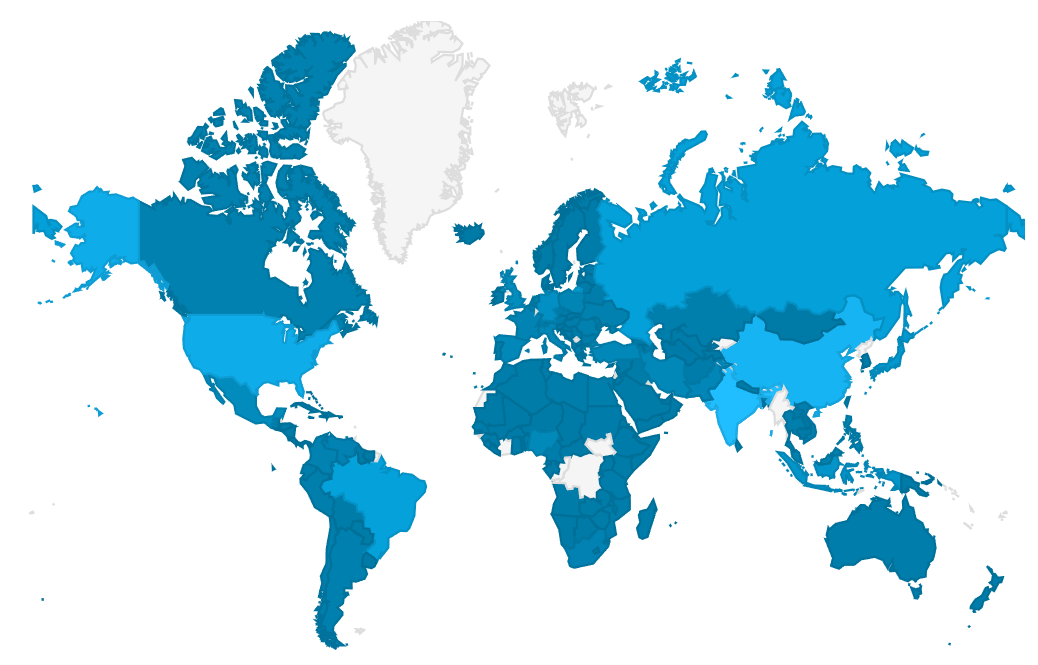
\includegraphics[width=\linewidth]{./map}
    \caption{Ursprung Daten (helleres Blau endspricht mehr Daten)}
    \label{fig:sub1}
\end{figure}

Die Aufzeichnungen reichen dabei von den frühesten Daten im Jahr 1743 bis zu den aktuellsten im Jahr 2015.

\subsection{Fehlende Daten und Ungenauigkeiten}
Bei unserer Analyse auf Duplikate stellten wir fest, dass 117 Städte im Datensatz doppelt oder mehrfach vorkommen. Dabei wurden Duplikate erkannt, falls die Daten zweier Städte vollständig identisch sind.  Diese doppelten Einträge sind vermutlich auf die Tatsache zurückzuführen, dass der Datensatz eine Zusammenstellung von 16 bereits bestehenden Datenarchiven darstellt. Im Datensatz sind zu den jeweiligen durchschnittlichen Temperaturen auch die durchschnittlichen Messunsicherheiten aufgeführt. Obwohl diese Unsicherheiten stetig abnehmen, stellen sie dennoch eine Herausforderung für die Vorhersagegenauigkeit dar (siehe Abbildung 2).
\begin{figure}[H]
    \flushleft
    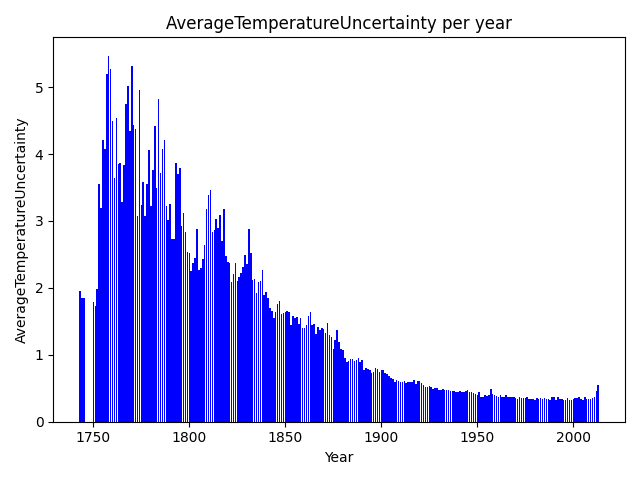
\includegraphics[width=\linewidth]{./Uncertainty_per_year}
    \label{fig:sub2}
    \caption{Messunsicherheit pro Jahr}
\end{figure}
dabei ist zu beachten, dass der exakte Messwert mit hoher Wahrscheinlichkeit eine geringere Abweichung aufweist als die Messunsicherheit. Daher ist der durchschnittliche Messfehler deutlich geringer als die Messunsicherheit.
Das bedeutet, das der Zufallsfaktor, der durch ungenaue Messungen entsteht und eine untere Schranke für die Vorhersagegenauigkeit bildet, nicht der angegebenen Messunsicherheit endspricht.


\subsection{Data-Loader Pipeline} % noch überarbeiten
Die Data-Loader Pipeline wurde implementiert, um Mini-Batches von Sequenzen von Datenpunkten gemäß den Anforderungen der Architekturen bereitzustellen. Dabei muss sichergestellt werden, dass Datenpunkte für die gesammte input länge von 70 Jahren(840 Monaten) und output länge von 25 Jahren(320 Monate) ohne Lücken vorhanden sind (siehe Abbildung 3).
\begin{figure}[H]
    \flushleft
    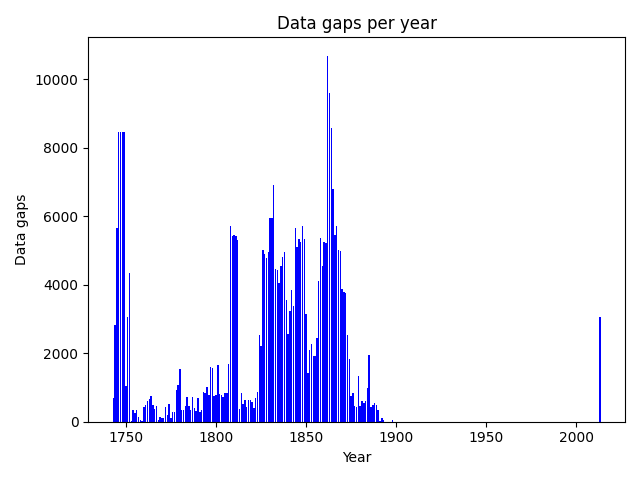
\includegraphics[width=\linewidth]{./Data_gaps}
    \label{fig:sub3}
    \caption{Messunsicherheit pro Jahr}
\end{figure}
Um die Effizienz des Trainings zu steigern, erfolgte die Extraktion der Daten aus den fünf CSV-Dateien, wobei für jeden Standort eine eigene Textdatei angelegt wurde. Zu Beginn wählten wir einen zufälligen Standort und einen zufälligen Zeitraum in dem 90 Jahre vollstänige Messwerte vohanden waren.
Später versuchten wir den Data-Loader weiter zu verbessern, dazu speicherten wir die gesamten Daten zunächst in Listen und führten die Suche nach passenden Zeiträumen einmalig am Anfang des Trainings durch. Diese Optimierung brachte jedoch nicht den gewünschten Effekt.

Die spätere Anwendung von Multiprocessing zur Ausführung des Data-Loaders auf bis zu 20 Prozessen gleichzeitig, beschleunigte den Data-Loader mit minimalem Aufwand um etwa das Zehnfache und erhöhte die Hardware-Auslastung merklich. Der Flaschenhals lag dabei im Arbeitsspeicher.

\section{Training-Procedure}

Um Klimaprognosen zu erstellen wurden die Architekturtypen MLP, ConvNet, LSTM und Transformer trainiert, auf einem Input von 70 Jahren(840 Monaten) eine Vorhersage für die Nächsten 25 Jahre(300) Monate zu treffen.
Im ersten Schritt wurde eine Grid Search durchgeführt, um optimale Modelle und deren Hyperparameter für die jeweiligen Architekturtypen zu aproximieren. 
Nach dieser automatisierten Suche wurde ein händisches Fine-Tuning durchgeführt, um die Leistung der Modelle weiter zu verbessern. 
Während des gesamten Prozesses wurde darauf geachtet, wie sich jede Architektur an die spezifischen Charakteristiken des Datensatzes anpasst und 
wie gut sie die Temperaturvorhersagen durchführen kann.

\subsection{Optimierung von Architekturen und Parametern}

Im Rahmen der Untersuchung wurden verschiedene Hyperparameterbetrachtet und optimiert, um die bestmöglichen Ergebnisse zu erzielen.
Dazu gehören zum einen allgemein Parameter wie etwa die Batchsize, Anzahl der Epochen, Steps pro Epoche, Anzahl der validierungs Steps und das Verhältniss von Trainingsdaten zu Validierungsdaten.
Weiterhin besitzen die genannten Architekturen auch eigene Charakteristiken, welche einen enormen Einfluss auf die Performance haben und dementsprechend im folgenden genauer untersucht werden.

\subsection{Allgemeine Parameter / Settings}

Da im Training als erstes eine Grid Search durchgeführt wurde und in dieser ausschließlich die Auswirkung der verschiedener Architekturen, Batch sizes und Learning rates auf den MAE untersucht wurden, mussten die restlichen Parameter zunächst festgelegt werden. Dabei wurde sich auf die bereits erwähnte Input- und Output-Länge, die Aufteilung des Datensatzes in 70 Prozent zum Trainieren und 30 Prozent zum Validieren und die Patience von 10 Epochen geeinigt. Durch die Patience wird sichergestellt, dass das Training erst nach 10 Epochen ohne eine Verbesserung des MAEs beendet wird. Des Weiteren wurden damit die Geschwindigkeit des Trainings vergleichbar bleibt die Steps/Epoche dynamisch an die Batch size angepasst, sodass unabhängig von der Batch Size, pro Epoche die gleiche Menge an Daten betrachtet werden. In der späteren Auswertung wird jedoch deutlich, dass selbst dieser Ansatz zur Vergleichbarkeit der Ergebnisse bei unterschiedlichen Batch-Größen nicht zwingend gerecht ist. Außerdem wurden Augmentation und Normalisierung in der Grid Search bisher noch nicht berücksichtigt.


\subsection{Grid Search}
\subsubsection{Training Mlps: }
Im Kontext von Multilayer-Perzeptronen (MLPs) spielen vor allem die Anzahl der Hidden Layer in Kombination mit der Dropout-Rate und die Anzahl der Neuronen pro Layer eine entscheidende Rolle bei der Optimierung. In der Grid Search wurden zunächst die folgenden Architekturen trainiert:
\begin{itemize}
    \item MLP1: 500, 200, 200, 400
    \item MLP2: 500, 500, 500, 500, 500, 500, 500, 500, 500
    \item MLP3: 1500, 1500, 1500, 1500, 1500
\end{itemize}
Das erste neuronale Netzwerk (NN) war ein Mehrschicht-Perzeptron (MLP) mit insgesamt 4 Schichten. Dabei umfasste die erste Schicht 500 Neuronen, die zweite 200 Neuronen und so weiter. Die Lernrate wurde dabei zwischen 0,001, 0,0005, 0,0001 und 0,000005 variiert. Die Batch-Größen wurden zwischen 25, 50, 100 und 200 gewählt.
\subsubsection{Training ConvNets: }
Für 1D-ConvNets sind insbesondere die Größe und Anordnung der Filter sowie deren Anzahl in den Convolutional Layern und dem darauf folgendem MLP von großer Bedeutung. 
In der Grid-Seach wurden zunächst die folgenden Architekturen trainiert:
\begin{itemize}
    \item ConvNet1: Anzahl: 10, 10, 10, Größe: 5,5,5 
    \item ConvNet2: Anzahl: 20, 20, 20, 20, 20, Größe 30, 30, 30, 30, 30
    \item ConvNet3: Anzahl: 50, 50, 50, 50, 50, Größe 10, 20, 20, 20, 10
    \item ConvNet4: Anzahl: 50, 50, 50,  Größe 10, 10, 10
\end{itemize}
Das ConvNet1 hat also 3 layer mit jeweils 10 Filtern der Größe 5.
Die Lernrate wurde zwischen 0.002, 0.001, 0.0004 und 0.0001 variiert. Die Batch-Größe wurde zwischen 25, 50, 75 und 100 gewählt.
Auf die ConvNet schichten folgte ein 4 Dense Layer der Form 400, 300, 200, 100 die in der Automatisierten Suche nicht weiter angepasst wurden.
\subsubsection{LSTMs (Long Short-Term Memory Networks) :}
Bei den LSTMs hingegen ist ein zentraler Parameter die Anzahl der Memory Units. In der Grid-Seach wurden zunächst die folgenden Architekturen trainiert:
\begin{itemize}
    \item LSTM1: 10, 10, 10, 10 Dense: 100,50
    \item LSTM2: 20, 20, 20, 20, 20, 20, 20, 20 Dense: 100, 90, 80, 70, 60, 50
    \item LSTM3: 30, 30, 30, 30, 30 Dense: 200,100
    \item LSTM4: 100, 100, 100, 100, 100 Dense: 500,250
\end{itemize}
So hat das erste LSTM 4 Layer mit jeweils 10 LSTM Units und 4 nachfolgende Dense Layer der Form 500, 250. Die lernrate wurde dabei zwischen 0,05, 0.03, 0.01 und 0.005 Variiert. Die Batch size zwischen 25, 50, 75 und 100.

\subsection{Fine Tuning}
Nach der Grid-Suche wurde ein zusätzliches Feintuning für die drei Architekturen MLP, ConvNet und LSTM durchgeführt. Dabei wurden die Parameter der jeweils besten Netzwerke weiter optimiert, und zusätzlich wurden bisher unbeachtete Parameter eingestellt. Für die Data Augmentation schien das Hinzufügen eines Gaus verteilten Zufallsfaktor nicht sehr sinnvoll stattdessen wurde eine Gaus-Verteilte Skalierung um einen Faktor zwischen 0.5 und 2 und ebenfalls eine Gausverteilte transformation um einen Faktor zwischen -10 und 10 vorgenommen. Somit konnten noch stärkere Temperatur extrema, eine Stätigere oder noch Variierendere Temperatur trainiert werden.
Aufgrund des Zeitaufwandes wurde für die Transformer keine Grid Search durchgeführt. Das finden einer möglichst performanten Architektur wurde hier ausschließlich durch menschliche Einstellungen bestimmt.  

\clearpage
\section{Results}

\subsection{Grid Search Ergebnisse}

Für alle MLPs sahen die Ergebnisse der Grid Search ähnlich aus hier beispielhaft für das MLP3 der MAE bei verschiedener Lernrate und Batch Size:
\begin{figure}[H]
    \flushleft
    \includegraphics[width=0.9\linewidth]{./MLP3}
    \label{fig:sub4}
    \caption{Grid Search MLP3}
\end{figure}
Der Fehler(MAE) war für alle drei Architekturen und jede gewählte Einstellung sehr niedrig. für die MLPs erzielten wir dabei einen minimalen Fehler von 0.88 mit dem MLP zwei mit folgendem Aufbau: 
\begin{figure}[H]
    \centering
    \includegraphics[width=0.7\linewidth]{./MLP2}
    \label{fig:sub5}
    \caption{Aufbau MLP2}
\end{figure}
Im fine Tuning hat sich dann herausgestellt, das mit einer etwas kleineren Architektur, längerem Training und einer größeren Batch size als aus der Grid search hervorgegangen ist eine Performance von MAE = 0.836 erreicht werden konnte. Dabei hat auch die Augmentation eine weitere Verbesserung erbracht.
Auch für die Conv nets waren die Ergebnisse äußerst Stabil. In dem Folgenden Diagramm ist der MAE ebispielhaft für das ConvNet2 über verschiedene Batch Sizes und Lernraten zu sehen:
\begin{figure}[H]
    \centering
    \includegraphics[width=0.9\linewidth]{./ConvNet2}
    \label{fig:sub6}
    \caption{Grid Search ConvNet2}
\end{figure}
Den besten MAE erreichte ConvNet1 dieser lag nach der Grid Search bei 0.86. Durch das Fine Tuning konnte die Genauigkeit auf bis 0.83 verbessert. dabei sorgten vor allem eine größere Batch Size eine angepasste Lernrate, längeres Training als auch Augementation für noch bessere Ergebnisse.
Das Traing für die LSTMs sah jedoch deutlich anders aus. Nicht alle Architekturen performten gut viele Trainings endeten mit einem MAE von 5 oder höher. Wie in dem besipielhaften Diagramm für Das LSTM4 zu sehen ist brachten nur wenige Konfigurationen erfolge:
\begin{figure}[H]
    \centering
    \includegraphics[width=0.9\linewidth]{./LSTM4}
    \label{fig:sub7}
    \caption{Grid Search LSTM4}
\end{figure}
Obwohl das beste LSTM(LSTM3) nach der Grid Search insgesamt das Netzwerk mit dem 89. besten MAE war, lag der Fehler bei etwa 1.1 Grad Celsius und konnte durch das Fine Tuning wiedererwartend auf bis 0.88 verbessert werden.

\subsubsection{Trainingsdauer}
Auch im Bezug auf die Trainingsdauer und Vorhersage geschwindigkeit lassen sich Unterschiede zwischen den verschiedenen Architekturen feststellen. 
Dies ist vorallem anhand der Komplexität der Modelle und den benötigten Berechnungen geschuldet, welche mehr oder weniger häufig und parallel ablaufen müssen.
So brauchten 1D-ConvNets als auch MLPs im Schnitt nur etwa 3 Sekunden pro Epoche wohingegen LSTMs als auch Transformer gerne mal 25 Sekunden brauchen.
Im Zusammenhang mit bis zu 300 Epochen, in denen Netzwerke trainiert wurden machen sich somit deutliche Differenzen sichtbar.

\subsubsection{Parameteranzahl}

In Anbetracht der verschiedenen Netzwerkarchitekturen und deren vergleichbaren Performance ergibt auch eine Analyse der Parameteranzahl Sinn. Bei größerer Anzahl an Parametern steigt ebenfalls der benötigte Speicherplatz für das jeweilige Model. Für manche Anwendungen kann der Speicherplatz ein limitierender Faktor sein während die größten Architekturen bis zu 500 Megabyte Speicherplatz benötigt haben, brauchen die kleinsten lediglich wenige hundert Kilobytes. 

Wie in der nachfolgenden Tabelle zu sehen besitzen Modelle der ConvNets überraschenderweise die meisten Parameter. Im Training der ConvNets ist aufgefallen, das bei Verwendung eines Global avarage poolings nach den Convolutional Layern also einer Durschnittsbildung über die gesamten Werte der Jeweiligen Feature Maps zu viele Daten über die Zeitreihen Verloren gehen. Daher haben wir uns entschieden ein Flatening einzubauen also die gesamten feature maps beizubehalten und als Input für die Dense Layers zu benutzen. Diese EnTscheidung hat dazu geführt, dass wir anstatt von etwa $800*20$ Daten auf 20 Durchschnitte abzubilden $800*20$ Outputs mit dem ersten Dense Layer verbunden haben, was bis zu etwa $800*50*400 = 16,000,000$ Verbindungen zwischen ConvNet und MLP geführt hat. 
Die LSTMs Weisen aufgrund der für die Inputs wiederverwendeten LSTM Einheiten eine vergleichsweise wenig Parameter auf. Die MLPs haben wie die ConvNets sehr viele Parameter da hier Jedes Neuron aus jeder Schicht mit der gesamten jeweiligen nächsten Schicht vebunden ist.
\begin{table}[htp]
    \centering
    \begin{tabular}{|c|c|c|c|c|}
    \hline
         Architektur & 1 & 2 & 3 & 4  \\
    \hline
         MLP & 761,600 &  2,574,800 & 10,717,800 & / \\
    \hline
          ConvNets& 3,544,380 &  5,840,000 & 15,707,050 & 16,541,950\\
    \hline
        LSTM & 24,450 &  71,470 & 89,720 & 613,450 \\
    \hline
    \end{tabular}
    \caption{Vergleich Anzahl Parameter}
    \label{tab:my_label}
\end{table}



\subsubsection{Performance und Stabilität im Training}
Auch wenn schlussendlich die besten Modelle der vier Architekturen ähnlich gut performen gibt es trotzdem Unterschiede in dem Verlauf und der Anpassung der Modelle an die Daten. Wie schon zuvor erwähnt haben die MLP als auch die ConvNets schon bei einer geringen Anzahl von Epochen direkt gute Ergebnisse mit MAEs im niedrigen einstelligen Bereich geliefert, während bei den LSTMs und den Transformern ein längeres Training (30-40 Epochen) zusammen mit einer genauen Auswahl an Architekturen notwendig war, bevor es zu zufriedenstellenden Ergebnissen kam.
\begin{figure}[H]
    \centering
    \includegraphics[width=0.9\linewidth]{./loss2}
    \label{fig:sub7}
    \caption{Loss Kurve ConvNet}
\end{figure}
Hier einmal eine Beispielhafte Loss Kurve eines ConvNets. Wie man sehen kann läuft das Training hier sehr schnell und Stabil während kein Overfitting als ein Auswendig lernen der Trainingsdaten geschieht.
Hier hingegen eine Loss-Curve eines LSTMs.
\begin{figure}[H]
    \centering
    \includegraphics[width=0.9\linewidth]{./loss3}
    \label{fig:sub7}
    \caption{Beispielhafte Loss Kurve LSTM}
\end{figure}



\subsection{Parameter Analyse}

\subsubsection{Early stopping und Modelsaving}
Durch die erwähnte Verwendung von Early stopping mit einer Patience von 10 wurde das Training der Modelle um einiges verkürtzt. So brauchten zum Beispiel MLPs bei der Grid Search nicht mehr 50 oder 100 Epochen durchlaufen werden, sondern es reichten schon ...  Epochen aus, bevor das jeweilige Modell sein Optimum ausreichend erreicht hatte. In Kombination dazu lohnt es sich zudem, mittels einer eigenen oder der von Tensorflow vordefinierten Methode nur die Modelle mit den besten Ergebnissen abzuspeichern, sodass es innerhalb der hier definierten Patience von 10 nicht zum Speichern von schlechteren Konfigurationen kommt (innerhalb von \texttt{tf.keras.callbacks.ModelCheckpoint} $\rightarrow$  \texttt{save\_best\_only=True}).

\subsubsection{Optimizer \& adaptive Learningrate}
Die verwendeten Optimizer waren Adam als auch SGD, wobei Adam in den meisten Fällen eine bessere Performance lieferte und somit bei dem größten Teil aller Modelle und vorallem bei den besten Modellen verwendet wurde.
Zusätzlich wurde eine adaptive Learningrate definiert, welche in Abhängigkeit von der Epoche eine abgeänderte Learningrate setzt. Dabei wurde zu Beginn auf die vom Adam Optimizer intern genutzte adaptive Learningrate zurückgegriffen, bis im weiteren Verlauf eine eigens definierte adaptive Learningrate verwendet wurde. Dabei konnten aber keine signifikanten Performanceunterschiede festgestellt werden. 

\subsubsection{Aktivierungsfunktionen}
Bei den Aktivierungsfunktionen wurden sowohl Selu \} als auch ReLu ($f(h)=max(h,0)$) verwendet, dabei gab es eine mit ReLu durchschnittlich bessere Performance  Allgemein lässt sich dazu sagen, dass sowohl Selu als auch ReLu die Linearität innerhalb des Netzwerkes brechen und somit zu einer höheren Kapazität und Komplexität des Netzwerkes beitragen, weshalb im Weiteren keine weiteren Aktivierungsfunktionen mehr betrachtet wurden.


\subsubsection{Overfitting, Augmentation, Normalisierung} 
Das Phänomen des Overfittings trat in keiner Phase der Datenverarbeitung dieses Datensatzes auf. Diese Unanfälligkeit lässt sich auf die beträchtliche Größe des Datensatzes zurückführen, der bereits eine ausreichende natürliche Varianz aufweist. Durch die Anwendung von Datenaugmentierung wird diese Varianz zusätzlich verstärkt.
Im Gegensatz dazu wurde bewusst auf die Normalisierung verzichtet. Bei einem derart begrenzten Wertebereich erschienen signifikante Verbesserungen durch Normalisierung unwahrscheinlich, während gleichzeitig die Interpretierbarkeit der Daten beeinträchtigt werden könnte. Der Datensatz umfasst dabei Temperaturdaten im Bereich von 40 bis -40 Grad Celsius.
\subsubsection{Input-Sequenzen}
Des Weiteren gab es keine umfänglichen Analysen zu variablen Input-Sequenzen, da die gewählten Skalen angepasst an den Datensatz zur zuverlässigen Vorhersagen von Temperaturdaten in einer Jahres-Skala dienen sollten und eine Input-Sequenz von zum Beispiel 8 bis 64 in diesem Kontext wenig Sinn zielführend wäre.


%%%%%%%%%%%%%%%%%%%%%%%%%%%%%%%%%%%%%%%%%%%%%%%%%%%%%%%%%%%%%%%

Bei 1D-ConvNets wurde die Auswirkung von Global Average Pooling und Flatten vor den Dense Layern untersucht. 
LSTM und Transformer wurden auf ihre spezifischen Eigenschaften und Fehlerquellen analysiert. 
Der Vergleich erfolgte durch Bewertung der qualitativen Anpassung und quantitativen Metriken wie dem Mean Absolute Error (MAE).


\begin{itemize}
    \item  gradient clipping gegen exploding gradientes bei RNN
    \item Binary Networks
    \item Positional Encoding (interessant für CONV, Transformer??)
    \item starke Varianz der Input-Sequenzlängen, da gesetzte größe einen begründeten Hintergrund hat 
    \item ...
\end{itemize}

\section{Conclusion}
\todo[size=\small]{TODO}

Die Anwendung neuronaler Netzwerke zur Vorhersage von Temperaturdaten über einen Zeitraum von hundert Jahren erweist sich als recht realistisch. Trotz der generell linearen Charakteristik der Vorhersagen liefern die Ergebnisse wertvolle Erkenntnisse bezüglich der Erkennung bekannter Klimatrends durch die Modelle und spiegeln ... 


\section{Citations and Bibliographies}

The use of \BibTeX\ for the preparation and formatting of one's
references is strongly recommended. Authors' names should be complete
--- use full first names (``Donald E. Knuth'') not initials
(``D. E. Knuth'') --- and the salient identifying features of a
reference should be included: title, year, volume, number, pages,
article DOI, etc.

The bibliography is included in your source document with these two
commands, placed just before the \verb|\end{document}| command:
\begin{verbatim}
  \bibliographystyle{ACM-Reference-Format}
  \bibliography{bibfile}
\end{verbatim}
where ``\verb|bibfile|'' is the name, without the ``\verb|.bib|''
suffix, of the \BibTeX\ file.

Citations and references are numbered by default. A small number of
ACM publications have citations and references formatted in the
``author year'' style; for these exceptions, please include this
command in the {\bfseries preamble} (before the command
``\verb|\begin{document}|'') of your \LaTeX\ source:
\begin{verbatim}
  \citestyle{acmauthoryear}
\end{verbatim}

  Some examples.  A paginated journal article \cite{Abril07}, an
  enumerated journal article \cite{Cohen07}, a reference to an entire
  issue \cite{JCohen96}, a monograph (whole book) \cite{Kosiur01}, a
  monograph/whole book in a series (see 2a in spec. document)
  \cite{Harel79}, a divisible-book such as an anthology or compilation
  \cite{Editor00} followed by the same example, however we only output
  the series if the volume number is given \cite{Editor00a} (so
  Editor00a's series should NOT be present since it has no vol. no.),
  a chapter in a divisible book \cite{Spector90}, a chapter in a
  divisible book in a series \cite{Douglass98}, a multi-volume work as
  book \cite{Knuth97}, a couple of articles in a proceedings (of a
  conference, symposium, workshop for example) (paginated proceedings
  article) \cite{Andler79, Hagerup1993}, a proceedings article with
  all possible elements \cite{Smith10}, an example of an enumerated
  proceedings article \cite{VanGundy07}, an informally published work
  \cite{Harel78}, a couple of preprints \cite{Bornmann2019,
    AnzarootPBM14}, a doctoral dissertation \cite{Clarkson85}, a
  master's thesis: \cite{anisi03}, an online document / world wide web
  resource \cite{Thornburg01, Ablamowicz07, Poker06}, a video game
  (Case 1) \cite{Obama08} and (Case 2) \cite{Novak03} and \cite{Lee05}
  and (Case 3) a patent \cite{JoeScientist001}, work accepted for
  publication \cite{rous08}, 'YYYYb'-test for prolific author
  \cite{SaeediMEJ10} and \cite{SaeediJETC10}. Other cites might
  contain 'duplicate' DOI and URLs (some SIAM articles)
  \cite{Kirschmer:2010:AEI:1958016.1958018}. Boris / Barbara Beeton:
  multi-volume works as books \cite{MR781536} and \cite{MR781537}. A
  couple of citations with DOIs:
  \cite{2004:ITE:1009386.1010128,Kirschmer:2010:AEI:1958016.1958018}. Online
  citations: \cite{TUGInstmem, Thornburg01, CTANacmart}. Artifacts:
  \cite{R} and \cite{UMassCitations}.

\section{Acknowledgments}

Identification of funding sources and other support, and thanks to
individuals and groups that assisted in the research and the
preparation of the work should be included in an acknowledgment
section, which is placed just before the reference section in your
document.

This section has a special environment:
\begin{verbatim}
  \begin{acks}
  ...
  \end{acks}
\end{verbatim}
so that the information contained therein can be more easily collected
during the article metadata extraction phase, and to ensure
consistency in the spelling of the section heading.

Authors should not prepare this section as a numbered or unnumbered {\verb|\section|}; please use the ``{\verb|acks|}'' environment.

\section{Appendices}

If your work needs an appendix, add it before the
``\verb|\end{document}|'' command at the conclusion of your source
document.

Start the appendix with the ``\verb|appendix|'' command:
\begin{verbatim}
  \appendix
\end{verbatim}
and note that in the appendix, sections are lettered, not
numbered. This document has two appendices, demonstrating the section
and subsection identification method.

\section{Multi-language papers}

Papers may be written in languages other than English or include
titles, subtitles, keywords and abstracts in different languages (as a
rule, a paper in a language other than English should include an
English title and an English abstract).  Use \verb|language=...| for
every language used in the paper.  The last language indicated is the
main language of the paper.  For example, a French paper with
additional titles and abstracts in English and German may start with
the following command
\begin{verbatim}
\documentclass[sigconf, language=english, language=german,
               language=french]{acmart}
\end{verbatim}

The title, subtitle, keywords and abstract will be typeset in the main
language of the paper.  The commands \verb|\translatedXXX|, \verb|XXX|
begin title, subtitle and keywords, can be used to set these elements
in the other languages.  The environment \verb|translatedabstract| is
used to set the translation of the abstract.  These commands and
environment have a mandatory first argument: the language of the
second argument.  See \verb|sample-sigconf-i13n.tex| file for examples
of their usage.

\section{SIGCHI Extended Abstracts}

The ``\verb|sigchi-a|'' template style (available only in \LaTeX\ and
not in Word) produces a landscape-orientation formatted article, with
a wide left margin. Three environments are available for use with the
``\verb|sigchi-a|'' template style, and produce formatted output in
the margin:
\begin{itemize}
\item {\verb|sidebar|}:  Place formatted text in the margin.
\item {\verb|marginfigure|}: Place a figure in the margin.
\item {\verb|margintable|}: Place a table in the margin.
\end{itemize}

%%
%% The acknowledgments section is defined using the "acks" environment
%% (and NOT an unnumbered section). This ensures the proper
%% identification of the section in the article metadata, and the
%% consistent spelling of the heading.
\begin{acks}
To Robert, for the bagels and explaining CMYK and color spaces.
\end{acks}

%%
%% The next two lines define the bibliography style to be used, and
%% the bibliography file.
\bibliographystyle{ACM-Reference-Format}
\bibliography{sample-base}

%%
%% If your work has an appendix, this is the place to put it.
\appendix

\section{Research Methods}

\subsection{Part One}

Lorem ipsum dolor sit amet, consectetur adipiscing elit. Morbi
malesuada, quam in pulvinar varius, metus nunc fermentum urna, id
sollicitudin purus odio sit amet enim. Aliquam ullamcorper eu ipsum
vel mollis. Curabitur quis dictum nisl. Phasellus vel semper risus, et
lacinia dolor. Integer ultricies commodo sem nec semper.

\subsection{Part Two}

Etiam commodo feugiat nisl pulvinar pellentesque. Etiam auctor sodales
ligula, non varius nibh pulvinar semper. Suspendisse nec lectus non
ipsum convallis congue hendrerit vitae sapien. Donec at laoreet
eros. Vivamus non purus placerat, scelerisque diam eu, cursus
ante. Etiam aliquam tortor auctor efficitur mattis.

\section{Online Resources}

Nam id fermentum dui. Suspendisse sagittis tortor a nulla mollis, in
pulvinar ex pretium. Sed interdum orci quis metus euismod, et sagittis
enim maximus. Vestibulum gravida massa ut felis suscipit
congue. Quisque mattis elit a risus ultrices commodo venenatis eget
dui. Etiam sagittis eleifend elementum.

Nam interdum magna at lectus dignissim, ac dignissim lorem
rhoncus. Maecenas eu arcu ac neque placerat aliquam. Nunc pulvinar
massa et mattis lacinia.

% \end{multicols}

\end{document}
\endinput
%%
%% End of file `sample-authordraft.tex'.
Besonders in den frühen Jahren der Temperaturaufzeichnung sind zudem Monate vorhanden, für die keine Werte protokolliert wurden.
